%---
\section{Intellectual Merit}

This proposal  is best categorized as an RI-1 Implementation Project (M1:IP). It seeks funding to support the development of infrastructure, the procurement of major equipment, and the construction and commissioning of the \DSk\ (\DSks) detector and \Urania\ plant.  This funding will constitute the majority of the capital support for U.S. involvement in the project.  The following will detail how the implementation of \DSk\ project will directly contribute to advances in fundamental science, engineering, technology, and other STEM related research and education.  


%---
\subsection{Scientific Justification}
%{Describe the potential for addressing one or more identified high-priority science goals within the relevant research community, the potential for advancing scientific discovery and the potential to significantly advance the Nation's research infrastructure.  Explain the unique research capabilities and lack of general availability of the proposed mid-scale infrastructure. Discuss the relationship to NSF's six Research Big Ideas, if applicable.}


There is strong evidence from astronomical and cosmological observations for the existence of dark matter in our Universe. Weakly Interacting Massive Particles (\WIMPs) are a well-motivated dark matter candidate that may have been produced in the early Universe but are so massive and weakly interacting that they have yet to be observed in a terrestrial experiment. The observation of \WIMPs\ with masses up to about 1 \si{\TeV\per\square\c} is a major objective of the experimental program at the High Luminosity Large Hadron Collider. Future high energy colliders like the FCC-$hh$ (Future Circular Collider) will be able to extend these searches up to the  \SI{10}{\TeV\per\square\c} mass range~\cite{CERN:2017cq}. Direct and indirect dark matter detection techniques allow for a search program complementary to future colliders. For example, the direct detection of dark matter via elastic scattering of galactic \WIMPs\ from a liquid argon target is a demonstrated technique capable of probing masses well above the reach of the LHC.

Liquid argon (\LAr) is a particularly favorable target for the detection of WIMPs thanks to its excellent event discrimination capabilities. Scintillation light initiated by particles recoiling from atomic electrons (\ERs), the primary source of background in a WIMP direct detection experiment, has a time constant of approximately a microsecond. This is in stark contrast to the nanosecond time constant of scintillation light emitted during an expected WIMP-nuclear recoil event (\NR). The \DEAP\ experiment has exploited this effect via pulse shape discrimination (\PSD) to achieve \ER\ background rejection of \DEAPPSDRejection~\cite{Amaudruz:2018gr,Ajaj:2019wi}. Additional event discrimination in an argon-based detector was demonstrated by the \DSf\ (\DSfs) experiment, which uses a two-phase time projection chamber to measure both the prompt argon scintillation light and the ionized electrons resulting from a particle interaction in the detector. This technique provides excellent position resolution and efficient detector fiducialization while maintaining \PSD\ capabilities~\cite{Agnes:2015gu,Agnes:2016fz}.  \DSfs\ has performed a blind analysis of their data and observed no background events over a run period in excess of two years~\cite{Agnes:2018ep}. In addition to sensitivity to WIMPs with masses above \DSkHighMassThreshold, the two-phase \DSfs\ detector has extended its reach to WIMP masses below \DSlLowMassThreshold\ by detecting single ionizaton electrons extracted from the liquid argon volume~\cite{Agnes:2018fg,Agnes:2018ft}.  With careful control of \ER\ background from local radioactivity and a reduction of the \ce{^39Ar} background, a \DSlApproxMassScale\ \LAr\ detector has the potential to reach the ``neutrino floor'' of solar neutrinos in this low-mass parameter space.


Given the potential reach of an argon-based detector, scientists from all of the major groups currently using \LAr\ to search for dark matter, including \ArDM, \DSfs, \DEAP, and \mCLEAN, have joined to form the Global Argon Dark Matter Collaboration (\GADMC) with a goal of building a series of future experiments that maximally exploit the advantages of \LAr\ as a detector target. 


%---
\subsubsection{\DSk: The High-Mass Search Program}
\label{sec:DSk}

\begin{figure}[t!]
\begin{center}
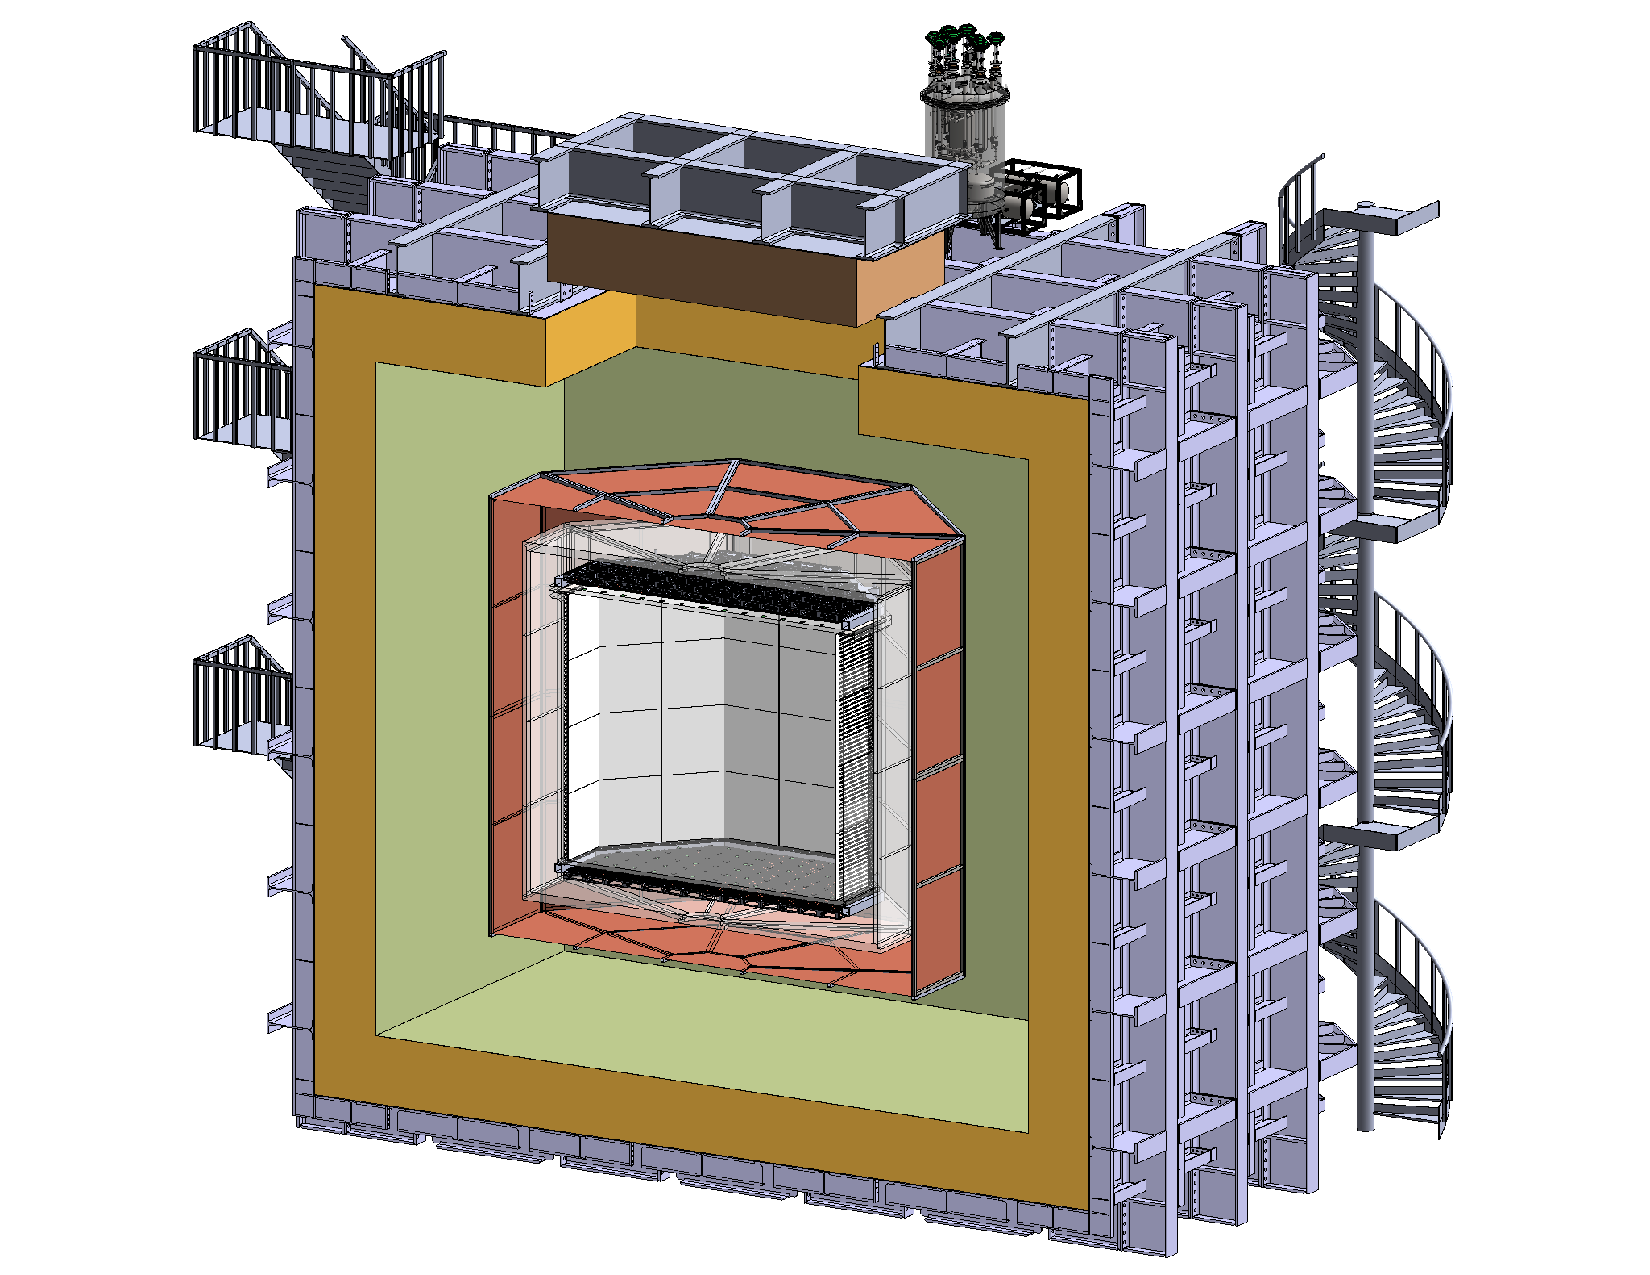
\includegraphics[width=\textwidth]{Figures/DSk3D.pdf}
\caption[Drawing of the \DSk\ detector.]{Drawing of the \DSks\ detector: the \PMMA\ \TPC\ filled with \UAr\ surrounded by the veto detector made of a \ce{Gd}-loaded \PMMA\ shell between two \AAr\ active layers, all contained within a membrane cryostat. The outer active argon layer is optically separated from the \AAr\ by a membrane.  For clarity, the mechanical supports holding the veto and \TPC\ are not shown.}
\label{fig:DSk3D}
\end{center}
\end{figure}


\begin{figure}[t!]
\begin{center}
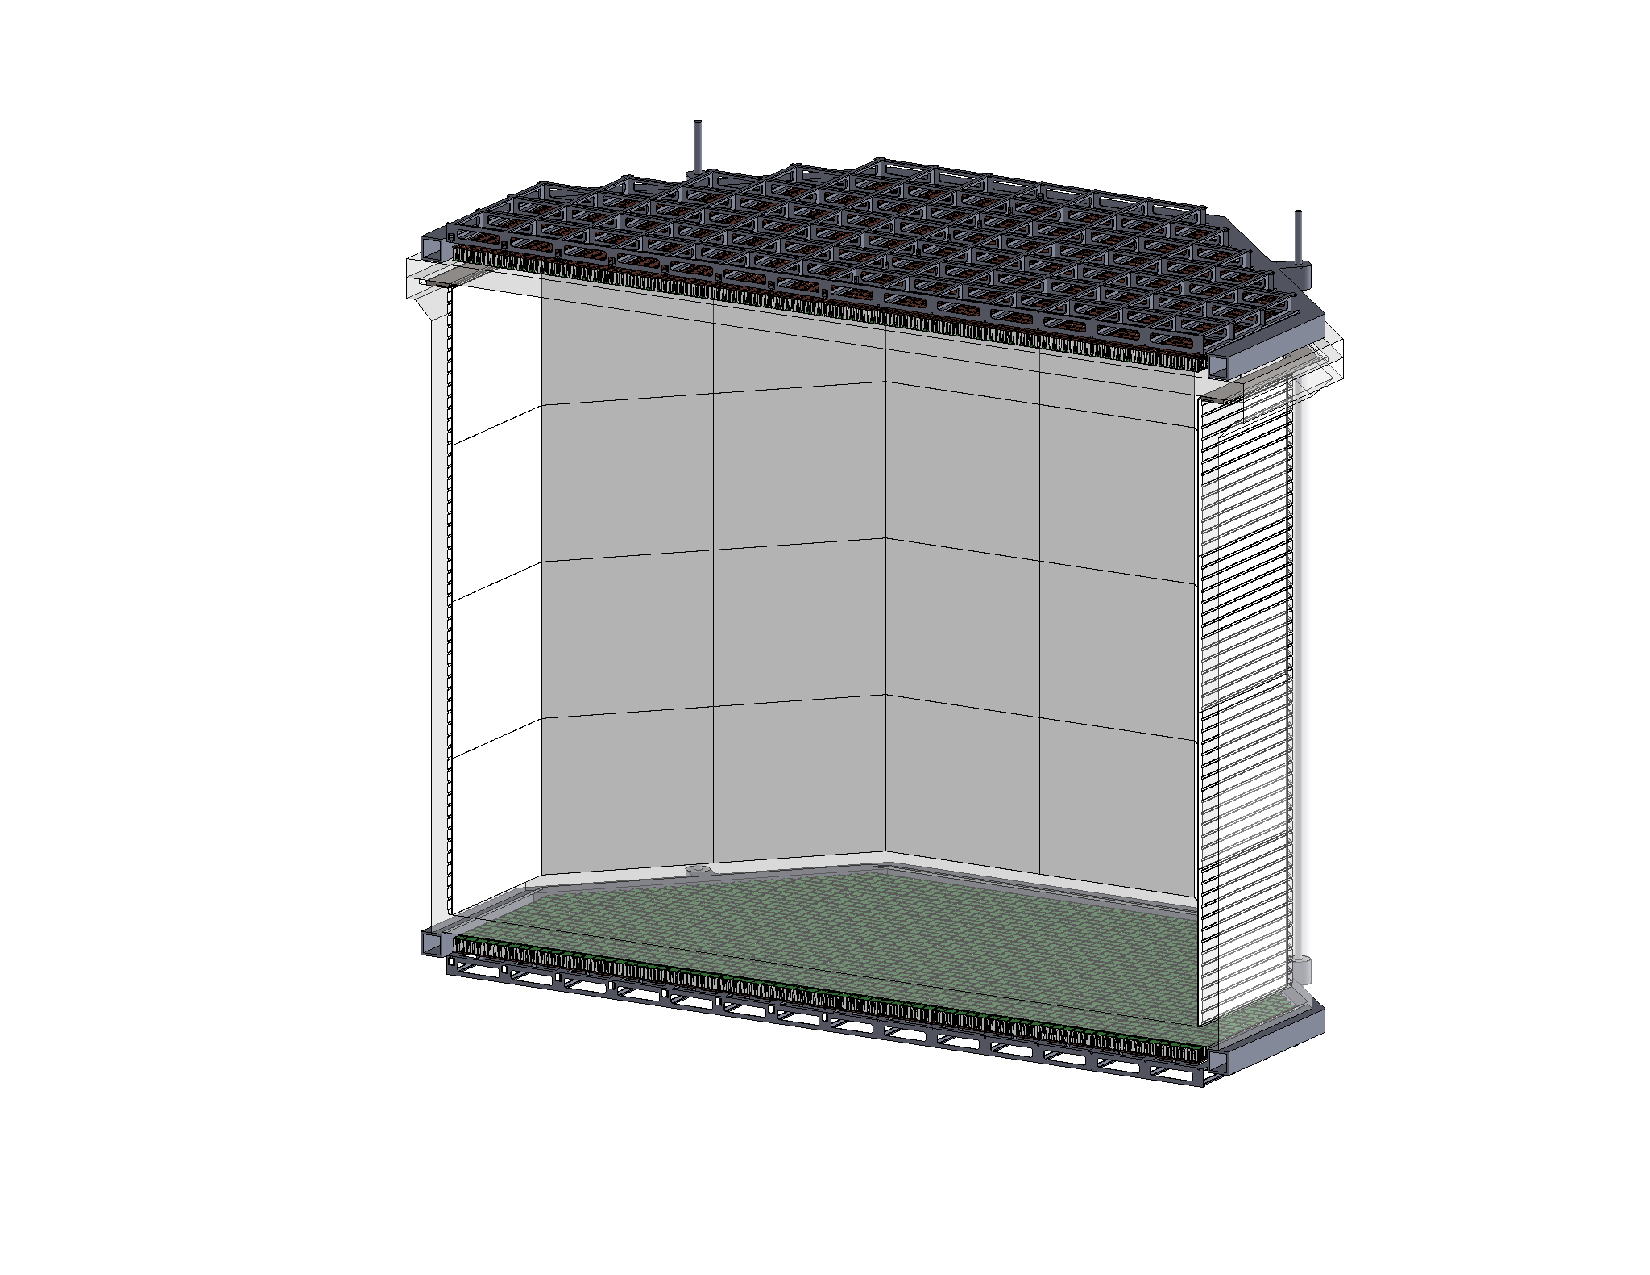
\includegraphics[width=0.8\textwidth]{Figures/TPC-acrylic-vessel-design.pdf}
\caption[Drawing of the \DSk\ \LArTPC.]{Drawing of the \DSk\ \LArTPC, detailing the \PMMA\ sealed vessel, \TPC\ field cage, and \DSkPdms\ support structure.    For clarity, the mechanical supports holding the \TPC\ and many other engineering details are not shown.}
\label{fig:DSk3D}
\end{center}
\end{figure}

The immediate objective of the \GADMC\ is construction of the \DSks\ two-phase \LAr\ detector, which will operate in Hall-C of the Gran Sasso National Laboratory (\LNGS).  \reffig{DSk3D} shows a 3D schematic of the \DSks\ detector. \DSks\ detector consists of two nested detectors housed within a \pDUNE-style membrane cryostat~\cite{Abi:2017wp,Acciarri:2016wz}.  

The inner detector is a dual-phase argon time projection chamber (\LArTPC) contained within a vessel made from ultra-pure  acrylic (\PMMA) and filled with \UAr.  The central active volume of the TPC is defined by eight vertical reflector panels and the top and bottom windows of the acrylic vessel. Instead of the traditional copper field cage rings and Indium-Tin-Oxide (\ITO) cathode and anode, \DSks\ will use poly(3,4-ethylenedioxythiophene) polystyrene sulfonate (also known as \PEDOT\ and commercialized under the name \Clevios~\cite{HeraeusDeutschlandGmbHandCOKg:2019wt}). All the TPC surfaces in contact with the active argon volume will be coated with  wavelength shifter tetraphenylbutadiene (\TPB) to convert \LAr\ scintillation light to a wavelength detectable by \SiPMs.  \DSkTilesNumber\ \SiPM-based PhotoDetector Modules (\DSkPdm) arrays will view the argon volume through the top and bottom windows of the acrylic vessel. The height of the \TPC\ is \DSkTPCHeight. The total mass of \LAr\ in the active volume is \DSkActiveMass.

The outer veto detector is made of a passive \ce{Gd}-loaded \PMMA\ shell surrounding the inner detector and between between two active \AAr\ layers.  The \ce{Gd}-loaded \PMMA\ shell moderates neutrons emitted from the \LAr\ \TPC\ until they capture on \ce{Gd}, resulting in the emission of multiple \grs.  The \grs\ interact in the \AAr\ layers and cause scintillation light that is detected by photodetectors, thereby providing an efficient veto of radiogenic neutrons that could result in a \NR\ in the TPC.  The \pDUNE-like cryostat will be surrounded by layers of plastic to moderate cosmogenic and radiogenic neutrons from the rocks surrounding Hall~C.


\begin{figure}[t!]
\begin{center}
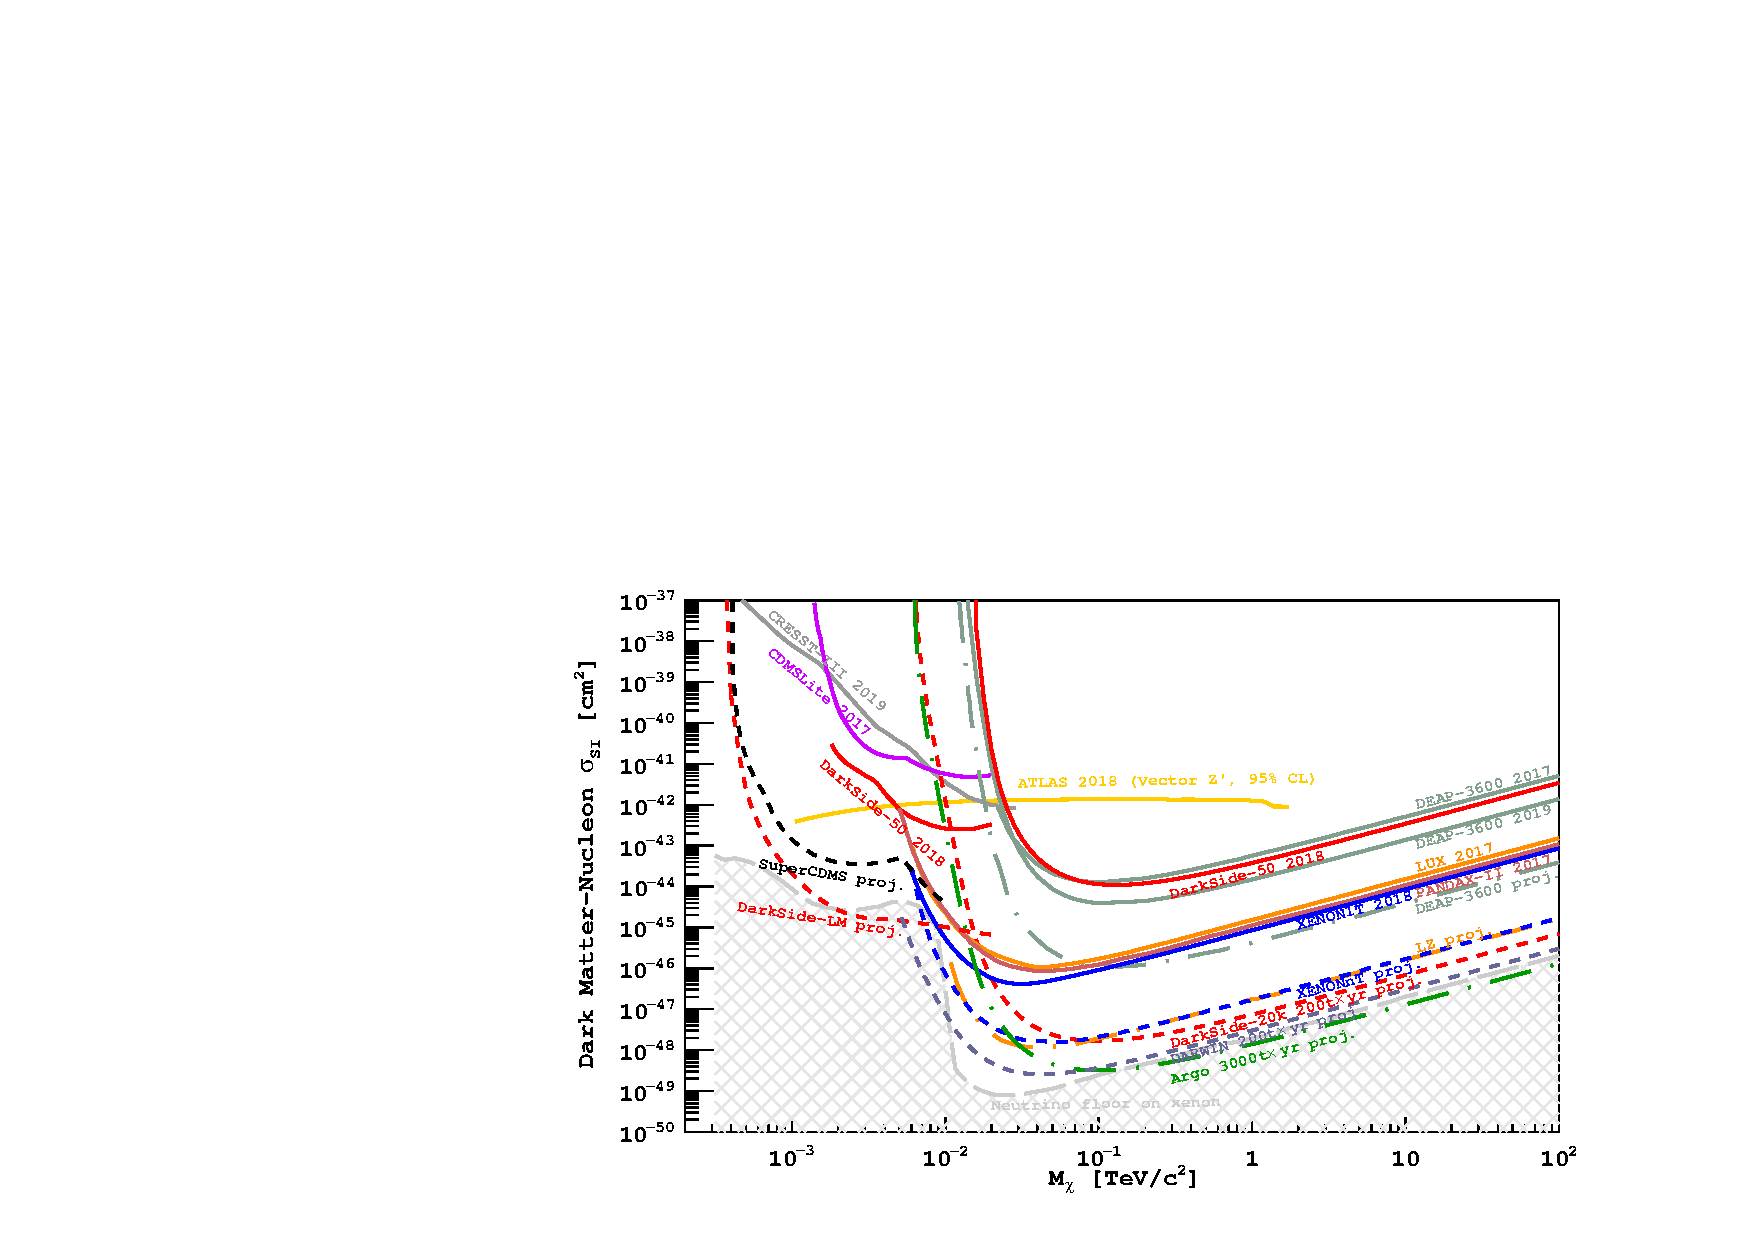
\includegraphics[width=\textwidth]{./Figures/DSklSensitivitySimplified.pdf}
\caption[Current \DM\ limits and sensitivities for future experiments.]
{\SI{90}{\percent} C.L. exclusion limits showing leading results from direct (continuous lines, Ref.~\cite{Angloher:2012kl,Akerib:2017kg,Cui:2017kg,Aprile:2018ct,Agnes:2018ep,Agnes:2018fg}) and accelerator-based dark matter searches (region above the yellow line \cite{TheATLASCollaboration:2018to}) compared with sensitivities of future germanium-, xenon-, and argon-based direct searches (dashed lines, Ref.~\cite{Nelson:2014wy,Kudryavtsev:2015hy,Aprile:2015wv,Boulay:2017tn,Agnese:2017fn} and this work).  The ``neutrino floor'' curve follows the definition of Ref.~\cite{Billard:2014cx}. The 95\% C.L. limit from the ATLAS Experiment is shown for a benchmark model in which Dirac-fermion WIMPs interact with ordinary matter via a vector mediator with coupling strengths to quarks, leptons and WIMPs of 0.25, 0.01, and 1, respectively~\cite{Abercrombie:2015to}.}
\label{fig:DSklSensitivitySimplified}
\end{center}
\end{figure}

The \DSks\ detector will have ultra-low backgrounds and the ability to measure its backgrounds {\it in situ}, resulting in an expected sensitivity to \WIMP-nucleon cross sections of \DSkSensitivityOneGeVUnit\ (\DSkSensitivityTenGeVUnit) for \WIMPMassOneTev\ (\WIMPMassTenTev) WIMPs following a \DSkRunTimePlannedVerbal\ run.  This projected sensitivity is a factor of~\DSkSensitivityImprovementOneTeV\ better than currently-published results above \WIMPMassOneTev\ and covers a large fraction of the parameter space currently preferred by supersymmetric models.

The sensitivity would further improve to \DSkExtendedSensitivityOneGeVUnit\ (\DSkExtendedSensitivityTenGeVUnit) for \WIMPMassOneTev\ (\WIMPMassTenTev) WIMPs for a \DSkExtendedRunTimePlannedVerbal\ run with a \DSkExtendedExposure\ exposure, see \reffig{DSklSensitivitySimplified}.  During the \DSkExtendedExposure\ exposure, \DSkNuInducedBackgroundExtendedExposureBare\ \NRs\ events are expected from the coherent scattering of atmospheric neutrinos, making \DSks\ the first ever direct dark matter detection experiment to reach this milestone.  The \DSks\ experiment is foreseen to begin operating in 2022 and will either detect \WIMP\ dark matter or exclude a large fraction of favored WIMP parameter space.

\DSks\ is designed to operate with zero backgrounds, meaning that all sources of instrumental background are reduced to \BackgroundFreeRequirement\ over a \DSkExtendedExposure\ exposure.  All background from minimum-ionizing radiation sources will be completely removed thanks to the combined action of \PSD\ of the primary scintillation pulse and comparison of the primary and secondary scintillation (see \refsec{IM-SC-XenonComp} for details on the suppression of background from \PP\ scatters on electrons and Ref.~\cite{Aalseth:2018gq} for that from \ce{^222Rn}, \ce{^220Rn}, and progenies).  \reftab{NeutronBackground} shows the expected radiogenic neutron background contributions of the various detector components following all \TPC\ and veto cuts for the full \DSks\ exposure.  The only remaining background for \WIMP\ searches will be the signal from the coherent scattering of atmospheric neutrinos on argon nuclei, with an expected \DSkNuInducedBackgroundExtendedExposureUnit\ over the \DSkExtendedExposure\ exposure.  \DSks\ will thus be the first experiment in a position to detect this important signal.

This outstanding sensitivity to coherent nuclear recoils will enables \DSks\ to detect a supernova neutrino burst coming from anywhere in the Milky Way Galaxy and, for a majority of the galaxy, clearly identify the neutronization burst. \DSks\ would perform a flavor-blind measurement of the total neutrino flux and average energy, setting an overall normalization that is not affected by neutrino oscillations. When combined with a flavor-specific measurement from a detector like Super-Kamiokande or DUNE, this observation could have sensitivity to the neutrino mass hierarchy. 

\begin{table*}[t]
\small
\begin{tabular}{lccccccc}
\hline \hline
\multirow{2}{*}{Material}
										&Mass			&\ce{^238U}		&\ce{^226Ra}	& $^{232}$Th	&Neutrons		&+\TPC			&+\TPC+veto\\
         								&[\si{tonne}]	&[\si{\milli\becquerel\per\kg}]
																		&[\si{\milli\becquerel\per\kg}]
																						&[\si{\milli\becquerel\per\kg}]
																										&[\DSkExtendedRunTimePlanned]$^{-1}$
																														&[\DSkExtendedExposure]$^{-1}$
																																		&[\DSkExtendedExposure]$^{-1}$\\
\hline
\TPC\ Vessel							&\num{2.7}		&\num{1.2E-2}	&\num{10}		& \num{4.1E-3}	&\num{5.7E2}	&\num{0.17}		&\num{1.7E-2}\\
\TPC\ SiPMs								&\num{0.12}		&-				& -				&-				&\num{5.4E3}	&\num{0.16}		&\num{1.6E-2}\\
\TPC\ Electronics						&\num{1.0}		&-				& -				&-				&\num{1.2E4}	&\num{0.36}		&\num{3.6E-2}\\
\TPC\ Mechanics							&\num{1.1}		&\num{3.9}		&\num{3.9}		&\num{1.9}		&\num{9.0E2}	&\num{1.8E-2} 	&\num{2.0E-3}\\
Veto \SiPMs+elec.						&\num{0.40}		&-				&-				&-				&\num{6.4E3} 	&\num{0.10}		&\num{1.0E-2}\\
Veto Acrylic							&\num{13}		&\num{1.2E-2}	&\num{10}		&\num{4.1E-3}	&\num{2.6E3}	&\num{4.2E-2} 	&\num{4.0E-3}\\
Veto Reflectors							&\num{1.0}		&\num{1.2E-2}	&\num{1.0}		&\num{4.1E-3}	&\num{2.0E2}	&\num{2.4E-2} 	&\num{2.0E-3}\\
Veto Steel								&\num{1.1}		&\num{3.9}		&\num{3.9}		&\num{1.9}		&\num{9.0E2}	&\num{1.4E-2}	&\num{1.0E-3}\\
\ce{Gd_2(SO_4)_3} $\alpha$'s on self	&\num{0.26}		&\num{7.0}		&\num{7.0}		&\num{0.2}		&\num{1.1E2}	&\num{2.0E-3}   &\num{<1.0E-3}\\
\ce{Gd_2(SO_4)_3} $\alpha$'s on \PMMA	&\num{0.26}		&\num{7.0}		&\num{7.0}		&\num{0.2}		&\num{3.6E2} 	&\num{6.0E-3}	&\num{1.0E-3}\\
Copper Cage								&\num{1.0}		&\num{0.30}		&\num{0.30}		&\num{2.0E-2}	&\num{6.0}		&\num{<1.0E-3}	&\num{<1.0E-3}\\
Cryostat Steel							&\num{250}		&\num{50}		&\num{1.0E3}	&\num{3.9}		&\num{1.0E6}	&-				&\num{<1.0E-3}\\
Cryostat Insulation 					&\num{40}		&\num{3E3}		&\num{8.0E3}	&\num{3.0E3}	&\num{8.0E7}	&-				&\num{<1.0E-3}\\
\hline
{\bf Total}								&				&				&				&				&				&\num[math-rm=\mathbf]{0.9}
																																		&\num[math-rm=\mathbf]{0.09}\\ 
\hline
\end{tabular}
\caption[Radiogenic neutrons sourced by the detector construction materials and background before and after cuts.]{Radiogenic neutrons sourced by the \LArTPC\ construction materials, veto and cryostat materials, with details of expected contamination levels, background after \TPC\ cuts, and residual background after combined \TPC\ and veto cuts, all relative to the full \DSkExtendedRunTimePlanned\ run time and the full fiducial \DSkExtendedExposure\ exposure.  The number of neutrons source is calculated from the expected contamination levels and material composition.  Note that no specific activity is reported for the \TPC\ \SiPMs\ and associated electronics: in this case the predicted neutron yield is the results of an extremely detailed calculation, accounting for the cumulative contribution of several tens of components, individually assayed.  The same consideration holds for the veto \SiPMs\ and electronics, whose contribution is reported in combination.  For neutrons due to ($\alpha$,n) reactions from $\alpha$'s from impurities in \ce{Gd_2(SO_4)_3}, the contribution is broken down between those due reactions on \ce{Gd} sulfate itself and those due to reactions in the \PMMA\ matrix containing the \ce{Gd} sulfate; the mass fraction of \ce{Gd} in the \GdAS\ \SI{1}{\percent}, for the anticipated \SI{2}{\percent} concentration by mass of \ce{Gd_2(SO_4)_3}.  (For ease of conversion: $\SI{1}{\ppt}(\ce{^238U}) \simeq \SI{1.2e-2}{mBq/kg}$; $\SI{1}{\ppt}(\ce{^232Th}) \simeq$ \SI{4.1e-3}{mBq/kg}.)}
\label{tab:NeutronBackground}
\end{table*}

 
This proposal requests funds for the U.S. contribution to the construction and commissioning of the \DSks\ detector at \LNGS\ and the Urania \UAr\ extraction facility, which will produce \UAr\ for the inner detector. There are six major areas that the U.S. NSF-supported groups will contribute to: the Urania plant installation and commissioning, photoelectronics development and fabrication, cryogenics and gas handling system design and fabrication, inner detector design and component fabrication, and development of calibrations sources and systems.  The responsibility of each NSF-supported group is outlined in the accompanying statements of work and other supplemental materials. These are critical components of the \DSk\ project that require the technical expertise and resources of the U.S. groups.


%---
\subsubsection{\DSl: The Low-Mass Search Program}
\label{sec:DSl}


In parallel to \DSks\ detector, the \GADMC\ will pursue the development of an approximately \DSlApproxMassScale\ detector specifically optimized for the detection of low-mass dark matter, \DSl\ (\DSls).  \DSls\ will achieve a lower energy threshold than \DSks\ by triggering on the electroluminescence signal from ionization electrons, thereby adding sensitivity to WIMP masses below \DSlLowMassThreshold\ at the expense of the \PSD\ power afforded by argon prompt scintillation light.  Without \PSD, contributors to the \ER\ background in \DSls\ must be reduced beyond the requirements of \DSks\ through careful detector design and material selection. While the \DSls\ experiment is outside the scope of this proposal, the implementation of \DSk\ project will have direct impacts on the technological advancements required to enable \DSls\ and the goal of reaching the neutrino floor for WIMP masses between \SI{1}{\GeV\per\c\squared} and \SI{10}{\GeV\per\c\squared}, see \reffig{DSklSensitivitySimplified}.  Among these are the development of low-background \DSkPdms~\cite{DIncecco:2018fx,DIncecco:2018hy} and the construction of the \Aria\ cryogenic distillation column, which will completely remove \ce{^85Kr} and reduce \ce{^39Ar} levels to the level of \SI{1}{\micro\becquerel\per\kg}.  The development of \DSls\ may exploit components of the \DSps\ detector under developed at \CERN.  Funding for the development, construction, commissioning, and operation of \DSls\ will be separately requested via alternative funding programs.


%---
\subsubsection{Argo}
\label{sec:Argo}

The ultimate objective of the GADMC is the construction of the \Argo\ detector, which will have a \GADMCFiducialMass\ fiducial mass and will push the experimental sensitivity to the point at which the coherent scattering of atmospheric neutrinos becomes a limiting background. The excellent \ER\ rejection possible in argon will eliminate backgrounds from solar neutrinos, which will extend the sensitivity of \Argo\ beyond that of technologies with more limited \ER\ discrimination. The throughput  of the \Urania\ plant and \Aria\ facility will enable \ArgoTotalMass\ of \UAr\ to be extracted and purified over a period of about \ArgoExtractionPeriod.  In addition to dark matter detection, such a large detector would also have excellent sensitivity to a neutrino burst associated with a galactic supernova.  If located at \SNOLAB\ or at similar depth, \Argo\ will also have the potential to observe \CNO\ neutrinos for the first time and solve the Solar Metallicity Problem~\cite{Franco:2016ex}.  While the construction of \Argo\ is not within the scope of this proposal, the implementation of  \DSk\ project will pave the way for the development of \Argo\ towards the end of the next decade. 

Combined \DSks, \DSls, and \Argo, will completely cover the spin-independent \WIMP\ hypothesis parameter space down to the neutrino floor for WIMP masses from \SI{1}{\GeV\per\square\c} to several hundreds of \si{\TeV\per\square\c}.


%---
\subsubsection{Comparison with Xenon-Based Experiments and the ``Neutrino Floor''}
\label{sec:IM-SC-XenonComp}

\begin{figure}
\begin{center}
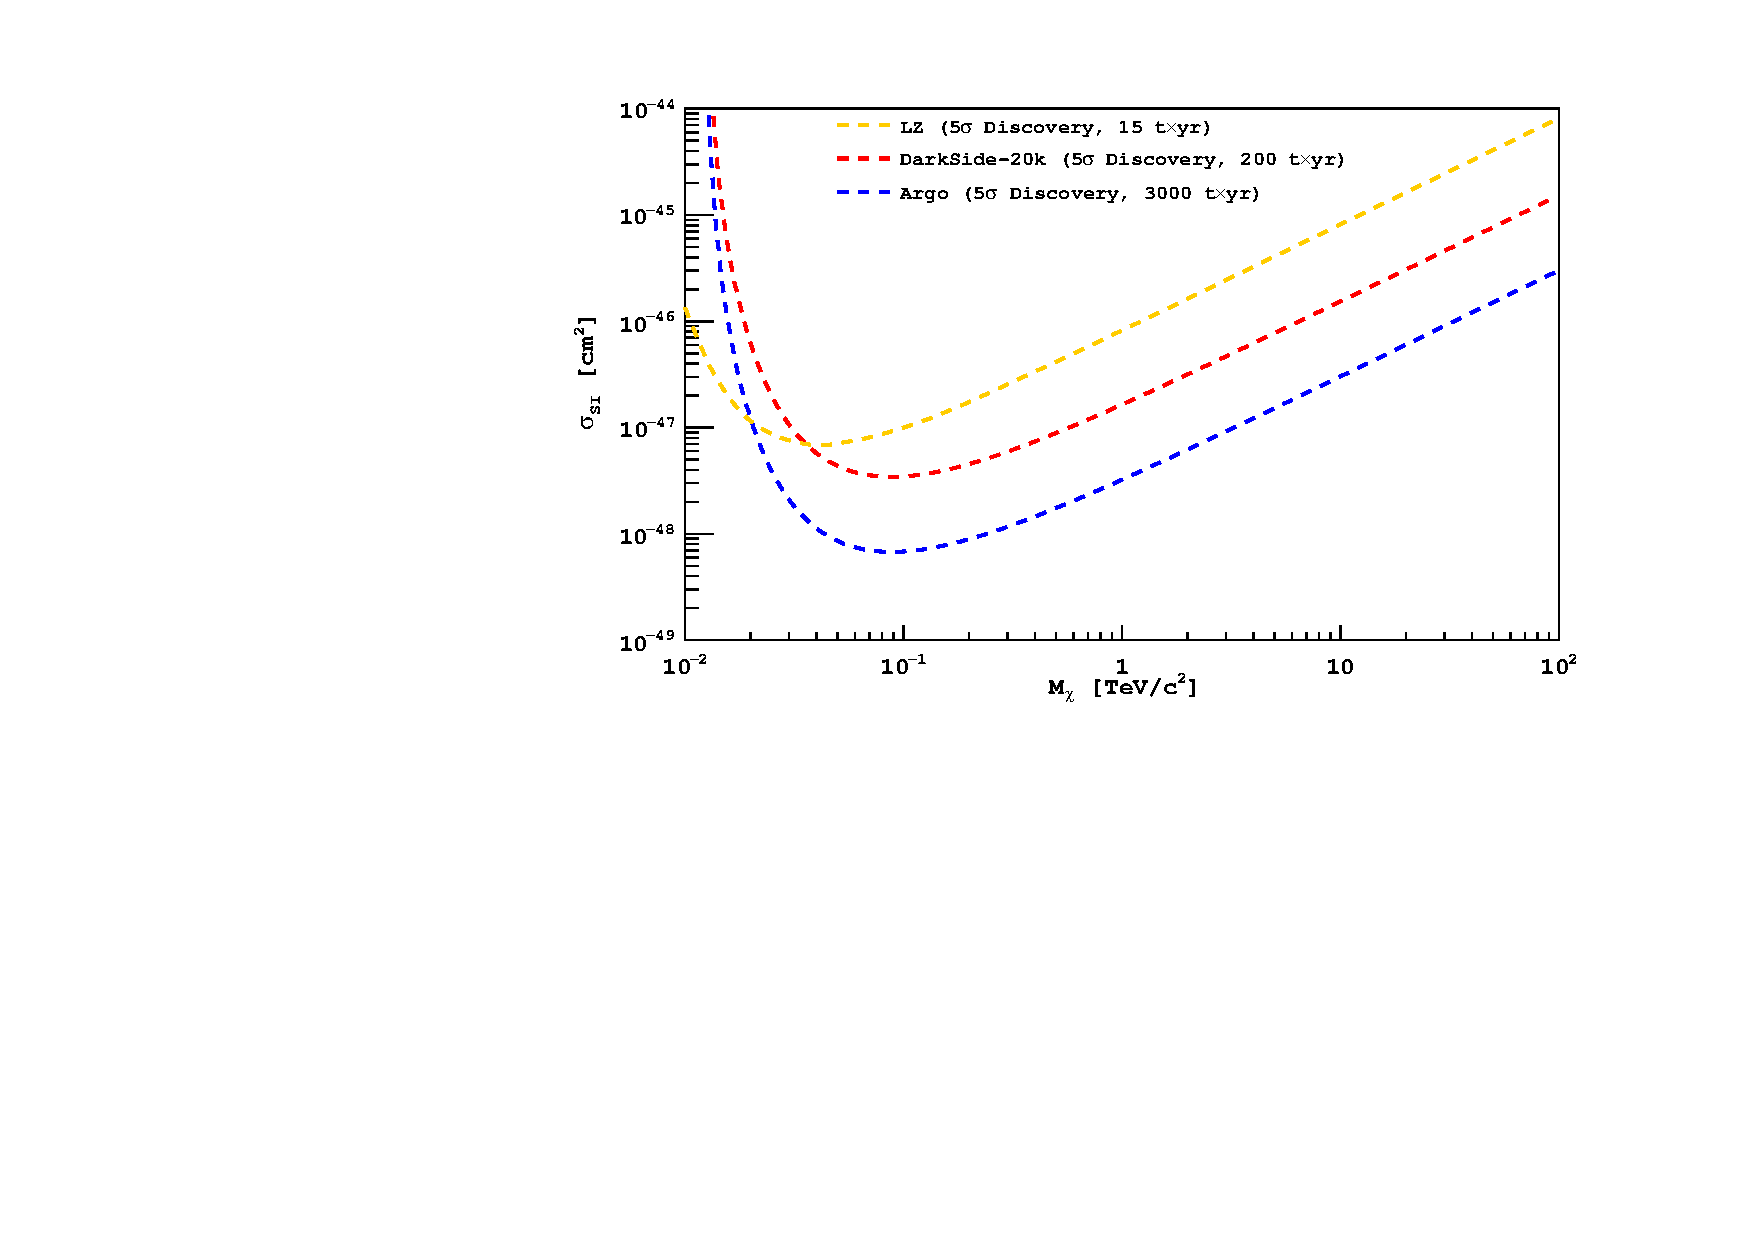
\includegraphics[width=\textwidth]{./Figures/NobleDiscoveryComp.pdf}
\caption{5$\sigma$ discovery potential of the leading future noble liquid dark matter searches.}
\label{fig:NobleDiscoveryComp}
\end{center}
\end{figure}

Next generation dark matter experiments will be sensitive to several sources of neutrinos via $\nu-e$ elastic scattering and coherent elastic neutrino scattering (\CEnNS) on nuclei (\NR). Atmospheric and diffuse supernovae neutrinos, which due to their high energies can produce \NRs\ in excess of \SI{20}{\keVr}, will be the dominant \CEnNS\ background contributor for WIMP masses above \DSkHighMassThreshold. Solar neutrinos are the main \CEnNS\ background for dark matter masses below \DSlLowMassThreshold. With  argon's ability to discriminate \ER\ from \NR\ to better than a part in \DEAPPSDRejection, \CEnNS\ represents the only irreducible background for a large exposure argon dark matter search. The neutrino background is exacerbated in liquid xenon detectors, which, due to their limited \ER\ rejection power, accept a non-negligible number of $\nu-e$ elastic scatters as signal. 

When calculating the discovery sensitivity of a large dark matter search experiment, one must fully account for the presence of neutrino-induced backgrounds.  We note that the position of the ``neutrino floor'', initially conceived as indicative of the maximum sensitivity attainable by an experiment in the presence of \CEnNS\ background, is critically dependent on the target, experimental technique, statistical analysis, neutrino flux uncertainty and theoretical cross section uncertainty. We therefore include a detailed accounting of the \CEnNS\ and $\nu-e$ backgrounds in the sensitivity and discovery potential curves shown in \reffig{DSklSensitivitySimplified} and \reffig{NobleDiscoveryComp}. We conservatively estimate a \SI{20}{\percent} uncertainty on the neutrino background for high-mass (\DSkHighMassThreshold) searches with \Argo.  This accounts for a \SI{15}{\percent} uncertainty on the atmospheric neutrino flux at mid-latitude locations, such as \SNOLAB\ or \LNGS, based on the latest data-driven models of cosmic primaries~\cite{Evans:2017hu} as well as models of solar cycle, seasonal, geographic, and geomagnetic dependence of the neutrino flux~\cite{Honda:2011ey,Barr:2006ih}.  Additionally, we account for a \SI{5}{\percent} theoretical uncertainty on the Standard Model interaction cross-section, driven by uncertainties on the nuclear form factor and the expected constraints that the COHERENT collaboration will place on non-Standard Model contributions using a \LAr\ target~\cite{Tayloe:2018jn}, which in turn is driven by their current \SI{10}{\percent} uncertainty on neutrino flux~\cite{Akimov:2017bs} and a \SI{6}{\percent} uncertainty on the \LAr\ response as measured by \SCENE~\cite{Cao:2015ks,Alexander:2013ke} and \ARIS~\cite{Agnes:2018cn}.  Planned improvements of COHERENT, including a sharper characterization of the neutrino flux and a measurement with a \LAr\ target, would further reduce the uncertainty on the neutrino background below \SI{10}{\percent}, strongly benefiting the \DSks, and \Argo\ experiments.

Within this framework, we calculate the 5$\sigma$ discovery potential for \DSks\ and \Argo\ and compare it with that of the near-future \LXe\ experiment LZ~\cite{Dobson:2018us}.  As seen from \reffig{NobleDiscoveryComp}, \DSks\ has significantly greater discovery potential than that of LZ.


%---
\subsubsection{New Technologies}
\label{sec:technologies}

The following technologies are key to the success of \DSk\ project and the long term scientific goals of the \GADMC. Their development will also have potentially wide-reaching effects within the physics community.

{\bf Low-Radioactivity Underground Argon with \Urania~\cite{Aalseth:2018gq}:} 
The \DSfs\ experiment established that \UAr\ is depleted of \ce{^39Ar} by a factor of approximately 1400, a sufficiently low rate to be deployed in a detector the size of \DSks. However, constructing \DSks\ will require that large amounts of \UAr\ be procured in a timely fashion. This will be accomplished by Urania, an argon extraction and purification plant capable of extracting \UraniaUArRate\ of \UAr.  The Urania plant is fully funded by the INFN and will be built by a contracted vendor following specifications established by the Urania Project team. The tender process for the plant's final design, construction, and shipment to the installation site in Cortez, Colorado, is underway and will conclude by the of end of July 2019 with the selection of a contractor.  The preparation of the extraction site, as well as the installation and commissioning of the plant, falls under the responsibility of the U.S. \NSF-supported groups.  The Urania \UAr\ extraction plant is projected to collect approximately \UraniaTotalDSkProduction\ of argon for use in \DSks\ detector by 2022 and could continue to produce underground argon for \Argo\ and other interested particle physics experiments that require \UAr\ to achieve their scientific objectives.  

{\bf Purification and Active Depletion with \Aria~\cite{Aalseth:2018gq}:}
The \Aria\ plant is a \SI{350}{\m} tall cryogenic distillation column that was designed to explore the possibility of chemically separating argon isotopes.  The construction of \Aria\ is fully supported by \INFN\ and Regione Autonoma della Sardegna. 

{\bf SiPM-based Cryogenic Photosensors~\cite{Aalseth:2018gq,DIncecco:2018hy,DIncecco:2018fx}:}
The development of low-background, large-area, cryogenic silicon photomultiplier (SiPM) detectors capable of replacing conventional photomultiplier tubes is critically important for achieving the desired sensitivity of \DSks\ and other large-scale \LAr-based experiments, including DUNE, and LXe-based detectors, such as \nEXO~\cite{Ostrovskiy:2015jl} and NEXT~\cite{Cebrian:2017dy,GomezCadenas:2016cm,Cebrian:2015du}.  The \DSks\ photodetector modules will be assembled at the Nuova Officina Assergi (\NOA), a dedicated cleanroom packaging facility that will have future utility for any experiment needing large volume silicon detector production.

{\bf \pDUNE\ Liquid Argon Cryostat~\cite{Abi:2017wp,Acciarri:2016wz}:}
\DSks\ detector will operate within a membrane cryostat filled with liquefied atmospheric argon, a technology initially developed at \CERN\ for \pDUNE. Eliminating the organic liquid scintillator veto used in \DSfs\ for the \AAr\ veto has several advantages. With the the \DSks\ \LArTPC\ directly immersed in \AAr, the massive stainless steel vacuum cryostat necessary for \DSfs, and its correspondingly large contribution of background events, can be replaced with a transparent, radio-pure \PMMA\ vessel. Photodetector modules can then be mounted outside of the \PMMA\ vessel, reducing their contribution to the background rate and simplifying their assembly strategy. The \pDUNE\ cryostat has the added advantage that it is scalable, making it a technology appropriate for \Argo.

{\bf Sealed \PMMA\ \TPC~\cite{Boulay:2012er,Nantais:2013jp,Amaudruz:2018gr}:}
The \DEAP\ collaboration has extensive experience developing large, radio-pure sealed \PMMA\ vessels. This technology will be used to build the vessel for the \DSks\ \LArTPC, eliminating the need for some of the most problematic radiogenic neutron contributors in \DSfs, most notably the stainless steel cryostat. The \PMMA\ vessel will also reduce the complexity of the \TPC\ assembly.

%---
\subsubsection{Community Recommendations}

In the U.S., the 2014 report of the Particle Physics Project Prioritization Panel (P5) ``Building for Discovery - Strategic Plan for U.S. Particle Physics in the Global Context''~\cite{ParticlePhysicsProjectPrioritizationPanel:2014td} states: {\it The experimental challenge of discovery and characterization of dark matter interactions with ordinary matter requires a multi-generational suite of progressively more sensitive and ambitious direct detection experiments.  This is a highly competitive, rapidly evolving field with excellent potential for discovery.  The second-generation direct detection experiments are ready to be designed and built, and should include the search for axions, and the search for low-mass ($<$10 GeV) and high-mass WIMPs.  Several experiments are needed using multiple target materials to search the available spin-independent and spin-dependent parameter space. }

P5 recommends: {\it Recommendation 20: Support one or more third-generation (G3) direct detection experiments, guided by the results of the preceding searches.  Seek a globally complementary program and increased international partnership in G3 experiments.}

In Europe, the ``European Astroparticle Physics Strategy 2017-2026''~\cite{AstroparticlePhysicsEuropeanConsortium:2017wy} authored by the ``Astroparticle Physics European Consortium'' (APPEC) states: {\it Medium-scale Dark Matter and neutrino experiments: APPEC considers as its core assets the diverse, often ultra-precise and invariably ingenious suite of medium-scale laboratory experiments targeted at the discovery of extremely rare processes.  These include experiments to detect the scattering of Dark Matter particles and neutrinoless double-beta decay, and direct measurement of neutrino mass using single-beta decay.  Collectively, these searches must be pursued to the level of discovery, unless prevented by an irreducible background or an unrealistically high demand for capital investment.}

APPEC then adds: {\it  For masses in excess of a few GeV, the best sensitivity to WIMPs is reached with detectors that use ultra-pure liquid noble-gas targets; such detectors include XENON1T (using 3.5 tons of xenon) and DEAP (using 3.6 tons of argon), which both started operating in 2016.  Their sensitivity can be further enhanced by increasing the target mass. A suite of smaller-scale experiments is exploring, in particular, low-mass WIMPs and other Dark Matter hypotheses such as those based on dark photons and axions.}

And it concludes: {\it APPEC encourages the continuation of a diverse and vibrant programme (including experiments as well as detector R\&D) searching for WIMPs and non-WIMP Dark Matter. With its global partners, APPEC aims to converge around 2019 on a strategy aimed at realising worldwide at least one `ultimate' Dark Matter detector based on xenon (in the order of 50 tons) and one based on argon (in the order of 300 tons), as advocated respectively by DARWIN and Argo.}


%---
\subsection{Research Community Benefits}

The \DSks\ project responds to two out of  NSF's Six Research Big Ideas.

{\bf Windows on the Universe:}
Recently, the Supernova Early Warning System (SNEWS) team submitted a proposal to the NSF Windows on the Universe solicitation for an upgrade to their system that enhance their capabilities.  \DSks\ was included in that proposal as a future partnering experiment that will work with the SNEWS network to detect galactic supernova neutrino bursts and provide an early warning of the incoming photon and gravitational wave signals.  The \DSks\ detector will have the unique ability to measure the supernova neutrinos in a flavor-blind way, meaning it will be able to constrain the total flux and the mean energy of the neutrinos over the duration of the burst.  This measurement, coupled with the neutrino measurements of other experiments and the photon and gravitational wave measurements, will provide a multi-messenger probe of a galactic supernova capable of differentiating between explosion mechanisms, characterizing neutron stars, studying black hole formation, answering general questions in particle physics and astrophysics, and providing new insight into neutrino oscillations.

{\bf Harnessing the Data Revolution:}
As in many of today's large-scale particle physics experiments, many petabytes of physics, calibration, and monte carlo simulation data will be collected, analyzed, and stored over the course of the 5 year \DSks\ operation. The collaboration is exploring new methods for storing and processing this data, including the use of machine learning algorithms for reconstruction, smart batch-data processing, and high-level physics analyses.  The implementation of the \DSks\ detector and its operation will expose a new generation of young researchers to big-data analysis. In particular, the \DSks\ data, due to the large number of expected \ER\ background events,  will have a massive class-imbalance. This creates an opportunity test new machine learning algorithms along with traditional analysis methods and compare their effectiveness.  This is a common problem within the information technology community, and \DSks\ will provide another opportunity to develop solutions in a basic research environment that will be broadly adaptable to other real-world problems.

{\bf Mid-scale Research Infrastructure:}
The \DSks\ project meets the criteria of an NSF Mid-scale Research Infrastructure outlined in \NSF's ``Bridging the Gap: Building a Sustained Approach to Mid-scale Research Infrastructure and Cyberinfrastructure at \NSF.'' It also benefits from the participation of and strong support of  international partners.

\DSks\ was jointly proposed to the US \NSF, the Italian \INFN, and \LNGS, the host laboratory, in December~2015.  The experiment was first reviewed by a joint panel charged by the Italian \INFN\ and the US \NSF.  The joint review was made possible by NSF statute NSF-14-1999 ``Dear Colleague Letter - International Activities within the Physics Division - Potential International Co-Review''~\cite{USNationalScienceFoundation:2014vy} following approval by the US State Department.  Following the first joint review, the experiment was also reviewed by the \INFN\ {\it Commissione Nazionale Seconda} (CSN2), the \INFN\ {\it Comitato Tecnico Scientifico} (CTS),  the \LNGS\ Scientific Committee, and the ``Particle Astrophysics -- Experiment'' panel of \NSF.  Following all reviews, the experiment was approved by \INFN\ and \LNGS\ in April~2017 and by \NSF\ in October~2017.  Following a meeting of participating international funding agencies and laboratories held at the Embassy of Canada in Rome in September~2017, the experiment was officially supported by three participating underground laboratories: the host laboratory \LNGS, Laboratorio Subterr\'aneo de Canfranc (\LSC), and \SNOLAB.

The \DSks\ experiment is hosted by \LNGS.  The \LNGS\ Scientific Committee, which meets two times per year, has oversight of the experiment and has assigned two Committee members as reviewers of \DSks.  The reviewers evaluate technical developments, schedule compliance, and collaboration issues, and report their findings to the \LNGS\ Scientific Committee.

\INFN\ has already provided most of the capital funds needed to support the \DSks\ project. R\&D and laboratory set-up costs have been covered by \INFN\ CSN2.  Additional funding in Italy, including support for the \Urania, \Aria, and \NOA\ facilities, comes from special and regional funds, the Ministero dello Sviluppo Economico (MISE), the Ministero dell'Istruzione, from the Universita e Ricerca (MIUR), the Regione Abruzzo, and the Regione Autonoma della Sardegna.  The Regione Autonoma della Sardegna and INFN instituted a Comitato di Indirizzo to manage the Aria project.  The Regione Autonoma della Sardegna and \INFN\ instituted a {\it Comitato di Indirizzo} to oversee and monitor the \Aria\ project.  Within \INFN, the experiment is regularly reviewed by the CSN2, which oversees technical developments and budget, collaboration, and schedule issues.  CSN2 appoints six permanent referees charged with the review and monitoring of \DSks.

Several groups from Canada joined the \DSs\ Collaboration in September~2017. They have secured funding for the large scale extraction of low-radioactivity argon from \CFI\ in Canada and funding for \DEAP\ R\&D from \NSERC.  An internal proposal for capital funds to support \DSks\ activities was submitted to \TRIUMF\ in October~2017 and was approved for funding.  A proposal to the Canadian \CFI\ for additional capital funds will be submitted in October 2019.  Recently, an agreement between \INFN\ and The Institute of High Energy Physics of the Chinese Academy of Sciences (\IHEP) reached an agreement to produce the acrylic material for both the \TPC\ and the veto detectors in China.  The \GADMC\ collaboration is currently composed of \num{59} institutions and \num{371} scientists from 15 nations: Brazil, Canada, China, France, Germany, Greece, Italy, Mexico, Poland, Romania, Russia, Spain, Switzerland, the United Kingdom, and the U.S.

{\bf NSF INCLUDES:}
The U.S. \DSk\ effort will leverage the involvement of Fort Lewis College in Durango, Colorado, to increase inclusion of underrepresented groups.  Since its founding in 1911, Fort Lewis College has demonstrated a unique commitment to the education of the local Native American population, in compliance with the deed that transferred the property of the former Fort Lewis from the Federal Government to the State of Colorado under condition that the land would be used for an educational institution, ``to be maintained as an institution of learning to which Indian students will be admitted free of tuition and on an equality with white students'' in perpetuity (Act of 61st Congress, 1911).  With this proposal, we request support to re-establish the Princeton-Gran Sasso Summer School for Physics. In the US, we will target high-school seniors and college freshman students from the Cortez-Durango area, offering them a period of study at Princeton, followed by a research period spent either at the Colorado Urania facility, the Aria facility in Sardinia, at LNGS, or at CERN.  This will expose them to otherwise unavailable on-site training and provide them with a network for pursuing job opportunities in the future, both through the project scientists and the companies partnered with the project.  The participation of students from the Cortez-Durango area may be complemented with that of high-school students from the Italian regions of the argon trail, {\it i.e.} Sardegna and Abruzzo. Funds for the participation of the Italian students will be independently sought from Italian government sources.